%! Author = thibaultchausson
%! Date = 11/12/2023

Pour réaliser cette métaheurisitique, nous devons fixer :
\begin{itemize}
    \item La taille de la liste taboue notée $T$, que nous définissions à 3
    \item Le voisinage sera un ensemble de permutations de deux éléments successifs ce qui donne $n - 1 = 10 -1 = 9$ en taille du voisinage.
\end{itemize}

Supposons que solution initiale $S_0$ soit

\begin{table}[!h]
    \centering
    \begin{tabular}{|c|c|c|c|c|c|c|c|c|c|c|c|}
        \hline
        \diagbox{Parents}{Cours} & 1  & 2 & 3 & 4 & 5  & 6 & 7 & 8 & 9  & 10 & Fitness \\
        \hline
        $S_0$                    & Ma & L & L & V & Me & J & J & V & Me & Ma & 6       \\
        \hline
    \end{tabular}
    \caption{$S_0$ recherche taboue}\label{tab:s-0-taboue}
\end{table}

Pour voir des cours bien équilibrés, nous décidons de répartir aléatoirement 2 cours par jour.

Nous reprenons la liste des v\oe ux des étudiants du tableau : \ref{tab:voeux-etudiant}.

Ainsi, nous avons :

\begin{table}[!h]
    \centering
    \begin{tabular}{|c|c|c|c|c|c|}
        \hline
        Jours & L    & Ma    & Me   & J    & V    \\
        \hline
        $S_0$ & 2, 3 & 1, 10 & 5, 9 & 6, 7 & 4, 8 \\
        \hline
    \end{tabular}
    \caption{$S_0$ initiale (jours)}\label{tab:s-0-taboue-jour}
\end{table}

$S_0$ a les conflits suivants :
\begin{enumerate}
    \item 2 cours en même temps donc $p_1 = 1$
    \item 2 cours en même temps donc $p_2 = 1$
    \item 2 cours en même temps donc $p_3 = 1$
    \item 0 cours en même temps donc $p_4 = 2$
    \item 1 cours en même temps donc $p_5 = 1$
\end{enumerate}
Donc, la fitness est de $6$.


\subsection{Exécutions}\label{subsec:executions}


\subsubsection{Intération 1}

\begin{table}[!h]
    \centering
    \begin{tabular}{|c|c|c|c|c|c|c|c|c|c|c|c|}
        \hline
        \diagbox{Parents}{Cours} & 1  & 2 & 3 & 4 & 5  & 6 & 7 & 8 & 9  & 10 & Fitness \\
        \hline
        $V_{1.1}$                & L  & Ma & L & V & Me & J & J & V & Me & Ma & 6       \\
        \hline
        $V_{1.2}$                & Ma & L  & L & V & Me & J & J & V & Me & Ma & 6       \\
        \hline
        $V_{1.3}$                & Ma & L  & V & L & Me & J & J & V & Me & Ma & 7       \\
        \hline
        $V_{1.4}$                & Ma & L  & L & Me & V & J & J & V & Me & Ma & 7       \\
        \hline
        $V_{1.5}$                & Ma & L  & L & V & J & Me & J & V & Me & Ma & 7       \\
        \hline
        $V_{1.6}$                & Ma & L  & L & V & Me & J & J & V & Me & Ma & 6       \\
        \hline
        $V_{1.7}$                & Ma & L  & L & V & Me & J & V & J & Me & Ma & 7       \\
        \hline
        $V_{1.8}$                & Ma & L  & L & V & Me & J & J & Me & V & Ma & 7       \\
        \hline
        $V_{1.9}$                & Ma & L  & L & V & Me & J & J & V & Ma & Me & 7       \\
        \hline
    \end{tabular}
    \caption{Le voisinage de l'itération 1}\label{tab:voisinage-1}
\end{table}


Solution retenue

\begin{table}[!h]
    \centering
    \begin{tabular}{|c|c|c|c|c|c|c|c|c|c|c|c|}
        \hline
        \diagbox{Parents}{Cours} & 1  & 2 & 3 & 4 & 5  & 6 & 7 & 8 & 9  & 10 & Fitness \\
        \hline
        $S_1$                    & Ma & L  & L & V & Me & J & V & J & Me & Ma & 7       \\
        \hline
    \end{tabular}
    \caption{Solution $S_1$}\label{tab:s-1}
\end{table}


\subsubsection{Intération 2}

\begin{table}[!h]
    \centering
    \begin{tabular}{|c|c|c|c|c|c|c|c|c|c|c|c|}
        \hline
        \diagbox{Parents}{Cours} & 1  & 2 & 3 & 4 & 5  & 6 & 7 & 8 & 9  & 10 & Fitness \\
        \hline
        $V_{2.1}$                & L  & Ma & L & V & Me & J & V & J & Me & Ma & 7       \\
        \hline
        $V_{2.2}$                & Ma & L  & L & V & Me & J & V & J & Me & Ma & 7       \\
        \hline
        $V_{2.3}$                & Ma & L  & V & L & Me & J & V & J & Me & Ma & 8       \\
        \hline
        $V_{2.4}$                & Ma & L  & L & Me & V & J & V & J & Me & Ma & 7       \\
        \hline
        $V_{2.5}$                & Ma & L  & L & V & J & Me & V & J & Me & Ma & 8       \\
        \hline
        $V_{2.6}$                & Ma & L  & L & V & Me & V & J & J & Me & Ma & 7       \\
        \hline
        $V_{2.7}$                & Ma & L  & L & V & Me & J & J & V & Me & Ma & 6       \\
        \hline
        $V_{2.8}$                & Ma & L  & L & V & Me & J & V & Me & J & Ma & 8       \\
        \hline
        $V_{2.9}$                & Ma & L  & L & V & Me & J & V & J & Ma & Me & 8       \\
        \hline
    \end{tabular}
    \caption{Le voisinage de l'itération 2}\label{tab:voisinage-2}
\end{table}

Solution retenue

\begin{table}[!h]
    \centering
    \begin{tabular}{|c|c|c|c|c|c|c|c|c|c|c|c|}
        \hline
        \diagbox{Parents}{Cours} & 1  & 2 & 3 & 4 & 5  & 6 & 7 & 8 & 9  & 10 & Fitness \\
        \hline
        $S_2$                    & Ma & L  & L & V & J & Me & V & J & Me & Ma & 8       \\
        \hline
    \end{tabular}
    \caption{Solution $S_2$}\label{tab:s-2}
\end{table}


\subsubsection{Intération 3}

\begin{table}[!h]
    \centering
    \begin{tabular}{|c|c|c|c|c|c|c|c|c|c|c|c|}
        \hline
        \diagbox{Parents}{Cours} & 1  & 2 & 3 & 4 & 5  & 6 & 7 & 8 & 9  & 10 & Fitness \\
        \hline
        $V_{3.1}$                & L  & Ma & L & V & J & Me & V & J & Me & Ma & 8       \\
        \hline
        $V_{3.2}$                & Ma & L  & L & V & J & Me & V & J & Me & Ma & 8       \\
        \hline
        $V_{3.3}$                & Ma & L  & V & L & J & Me & V & J & Me & Ma & 9       \\
        \hline
        $V_{3.4}$                & Ma & L  & L & J & V & Me & V & J & Me & Ma & 7       \\
        \hline
        $V_{3.5}$                & Ma & L  & L & V & Me & J & V & J & Me & Ma & 7       \\
        \hline
        $V_{3.6}$                & Ma & L  & L & V & J & V & Me & J & Me & Ma & 8       \\
        \hline
        $V_{3.7}$                & Ma & L  & L & V & J & Me & J & V & Me & Ma & 7       \\
        \hline
        $V_{3.8}$                & Ma & L  & L & V & J & Me & V & Me & J & Ma & 7       \\
        \hline
        $V_{3.9}$                & Ma & L  & L & V & J & Me & V & J & Ma & Me & 8       \\
        \hline
    \end{tabular}
    \caption{Le voisinage de l'itération 3}\label{tab:voisinage-3}
\end{table}

Solution retenue

\begin{table}[!h]
    \centering
    \begin{tabular}{|c|c|c|c|c|c|c|c|c|c|c|c|}
        \hline
        \diagbox{Parents}{Cours} & 1  & 2 & 3 & 4 & 5  & 6 & 7 & 8 & 9  & 10 & Fitness \\
        \hline
        $S_3$                    & Ma & L  & V & L & J & Me & V & J & Me & Ma & 9       \\
        \hline
    \end{tabular}
    \caption{Solution $S_3$}\label{tab:s-3}
\end{table}


\subsubsection{Intération 4}

\begin{table}[!h]
    \centering
    \begin{tabular}{|c|c|c|c|c|c|c|c|c|c|c|c|}
        \hline
        \diagbox{Parents}{Cours} & 1  & 2 & 3 & 4 & 5  & 6 & 7 & 8 & 9  & 10 & Fitness \\
        \hline
        $V_{4.1}$                & L  & Ma & V & L & J & Me & V & J & Me & Ma & 9       \\
        \hline
        $V_{4.2}$                & Ma & V  & L & L & J & Me & V & J & Me & Ma & 9       \\
        \hline
        $V_{4.3}$                & Ma & L  & L & V & J & Me & V & J & Me & Ma & 8       \\
        \hline
        $V_{4.4}$                & Ma & L  & V & J & L & Me & V & J & Me & Ma & 8       \\
        \hline
        $V_{4.5}$                & Ma & L  & V & L & Me & J & V & J & Me & Ma & 8       \\
        \hline
        $V_{4.6}$                & Ma & L  & V & L & J & V & Me & J & Me & Ma & 9       \\
        \hline
        $V_{4.7}$                & Ma & L  & V & L & J & Me & J & V & Me & Ma & 8       \\
        \hline
        $V_{4.8}$                & Ma & L  & V & L & J & Me & V & Me & J & Ma & 8       \\
        \hline
        $V_{4.9}$                & Ma & L  & V & L & J & Me & V & J & Ma & Me & 9       \\
        \hline
    \end{tabular}
    \caption{Le voisinage de l'itération 4}\label{tab:voisinage-4}
\end{table}

Solution retenue

\begin{table}[!h]
    \centering
    \begin{tabular}{|c|c|c|c|c|c|c|c|c|c|c|c|}
        \hline
        \diagbox{Parents}{Cours} & 1  & 2 & 3 & 4 & 5  & 6 & 7 & 8 & 9  & 10 & Fitness \\
        \hline
        $S_4$                    & Ma & L  & V & L & J & Me & V & J & Ma & Me & 9       \\
        \hline
    \end{tabular}
    \caption{Solution $S_4$}\label{tab:s-4}
\end{table}


\subsubsection{Intération 5}


\begin{table}[!h]
    \centering
    \begin{tabular}{|c|c|c|c|c|c|c|c|c|c|c|c|}
        \hline
        \diagbox{Parents}{Cours} & 1  & 2 & 3 & 4 & 5  & 6 & 7 & 8 & 9  & 10 & Fitness \\
        \hline
        $V_{5.1}$                & L  & Ma & V & L & J & Me & V & J & Ma & Me & 10      \\
        \hline
        $V_{5.2}$                & Ma & V  & L & L & J & Me & V & J & Ma & Me & 9       \\
        \hline
        $V_{5.3}$                & Ma & L  & L & V & J & Me & V & J & Ma & Me & 8       \\
        \hline
        $V_{5.4}$                & Ma & L  & V & J & L & Me & V & J & Ma & Me & 8       \\
        \hline
        $V_{5.5}$                & Ma & L  & V & L & Me & J & V & J & Ma & Me & 9       \\
        \hline
        $V_{5.6}$                & Ma & L  & V & L & J & V & Me & J & Ma & Me & 9       \\
        \hline
        $V_{5.7}$                & Ma & L  & V & L & J & Me & J & V & Ma & Me & 8       \\
        \hline
        $V_{5.8}$                & Ma & L  & V & L & J & Me & V & Ma & J & Me & 8       \\
        \hline
        $V_{5.9}$                & Ma & L  & V & L & J & Me & V & J & Me & Ma & 9       \\
        \hline
    \end{tabular}
    \caption{Le voisinage de l'itération 5}\label{tab:voisinage-5}
\end{table}


Solution retenue

\begin{table}[!h]
    \centering
    \begin{tabular}{|c|c|c|c|c|c|c|c|c|c|c|c|}
        \hline
        \diagbox{Parents}{Cours} & 1  & 2 & 3 & 4 & 5  & 6 & 7 & 8 & 9  & 10 & Fitness \\
        \hline
        $S_5$                    & L  & Ma & V & L & J & Me & V & J & Ma & Me & 10      \\
        \hline
    \end{tabular}
    \caption{Solution $S_5$}\label{tab:s-5}
\end{table}


\subsubsection{Bilan}

En 5 itération

\begin{table}[!h]
    \centering
    \begin{tabular}{|c|c|c|c|c|c|c|c|c|c|c|c|}
        \hline
        \diagbox{Parents}{Cours} & 1  & 2 & 3 & 4 & 5  & 6 & 7 & 8 & 9  & 10 & Fitness \\
        \hline
        $S_5$                    & L  & Ma & V & L & J & Me & V & J & Ma & Me & 10      \\
        \hline
    \end{tabular}
    \caption{Solution $S_5$ finale}\label{tab:s-5-final}
\end{table}


\begin{figure}[!h]
    \begin{center}
        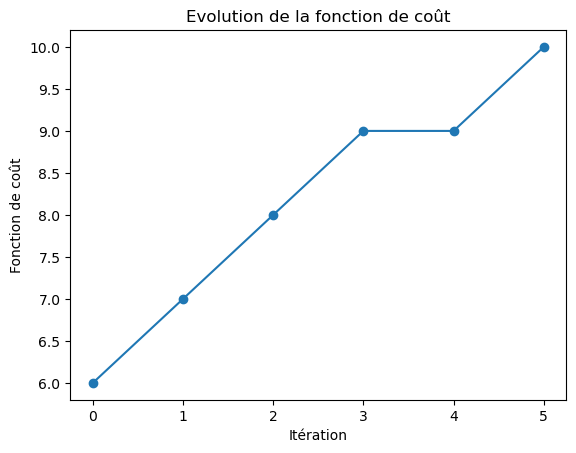
\includegraphics[scale=0.8]{ressources/taboueCoutGraph}
        \caption{Évolution de la fitness \label{fig:evolFitnessTaboue}}
    \end{center}
\end{figure}